\documentclass[]{beamer}
% Class options include: notes, notesonly, handout, trans,
%                        hidesubsections, shadesubsections,
%                        inrow, blue, red, grey, brown

% Theme for beamer presentation.
\usepackage{beamerthemesplit} 
% Other themes include: beamerthemebars, beamerthemelined, 
%                       beamerthemetree, beamerthemetreebars  

\title{Robustness in White Rabbit}    % Enter your title between curly braces
\author{Maciej Lipinski, Cesar Prados}                 % Enter your name between curly braces
\institute{CERN \&  GSI}      % Enter your institute name between curly braces
\date{\today}                    % Enter the date or \today between curly braces

\usepackage{graphicx}
\usepackage{epstopdf}

\graphicspath{ {../../figures/} }
\begin{document}

% Creates title page of slide show using above information
\begin{frame}
  \titlepage{Robustness in White Rabbit}
\end{frame}
\note{Talk for 30 minutes} % Add notes to yourself that will be displayed when
                           % typeset with the notes or notesonly class options

\section*{Outline}
\begin{frame}
  \tableofcontents
\end{frame}

\begin{frame}
\begin{figure}[tbp] % float placement: (h)ere, page (t)op, page (b)ottom, other (p)age
  \centering
  % file name: E:/Moje Dokumenty/PW/doktorat/PhD_project/whireRabbit/repo/trunk/documentation/presentations/robustness/hierarchy.pdf
  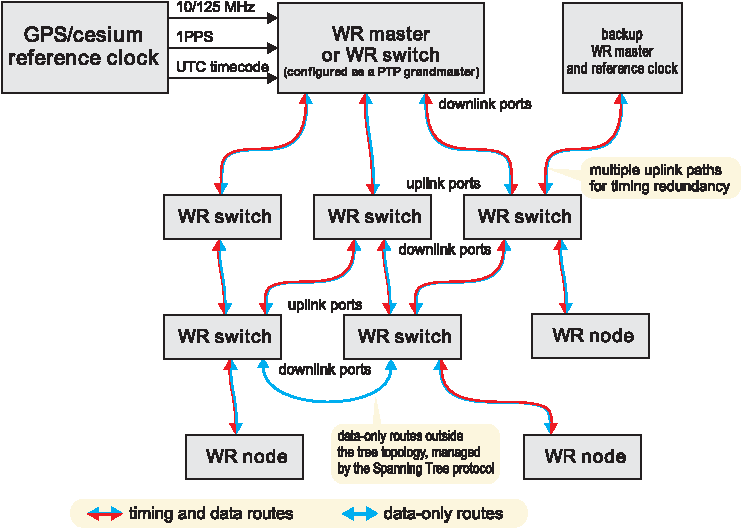
\includegraphics[height=2.65in,keepaspectratio]{network/hierarchy.pdf}
  %\caption{Overview of White Rabbit Network}
  \label{fig:hierarchy}
\end{figure}

\end{frame}

\section{Robustness Layer 1}

\subsection{Clock Recovery...holdover}

\begin{frame}
  \frametitle{Clock Recovery...holdover}   % Insert frame title between curly braces
\begin{figure}[tbp] % float placement: (h)ere, page (t)op, page (b)ottom, other (p)age
  \centering

  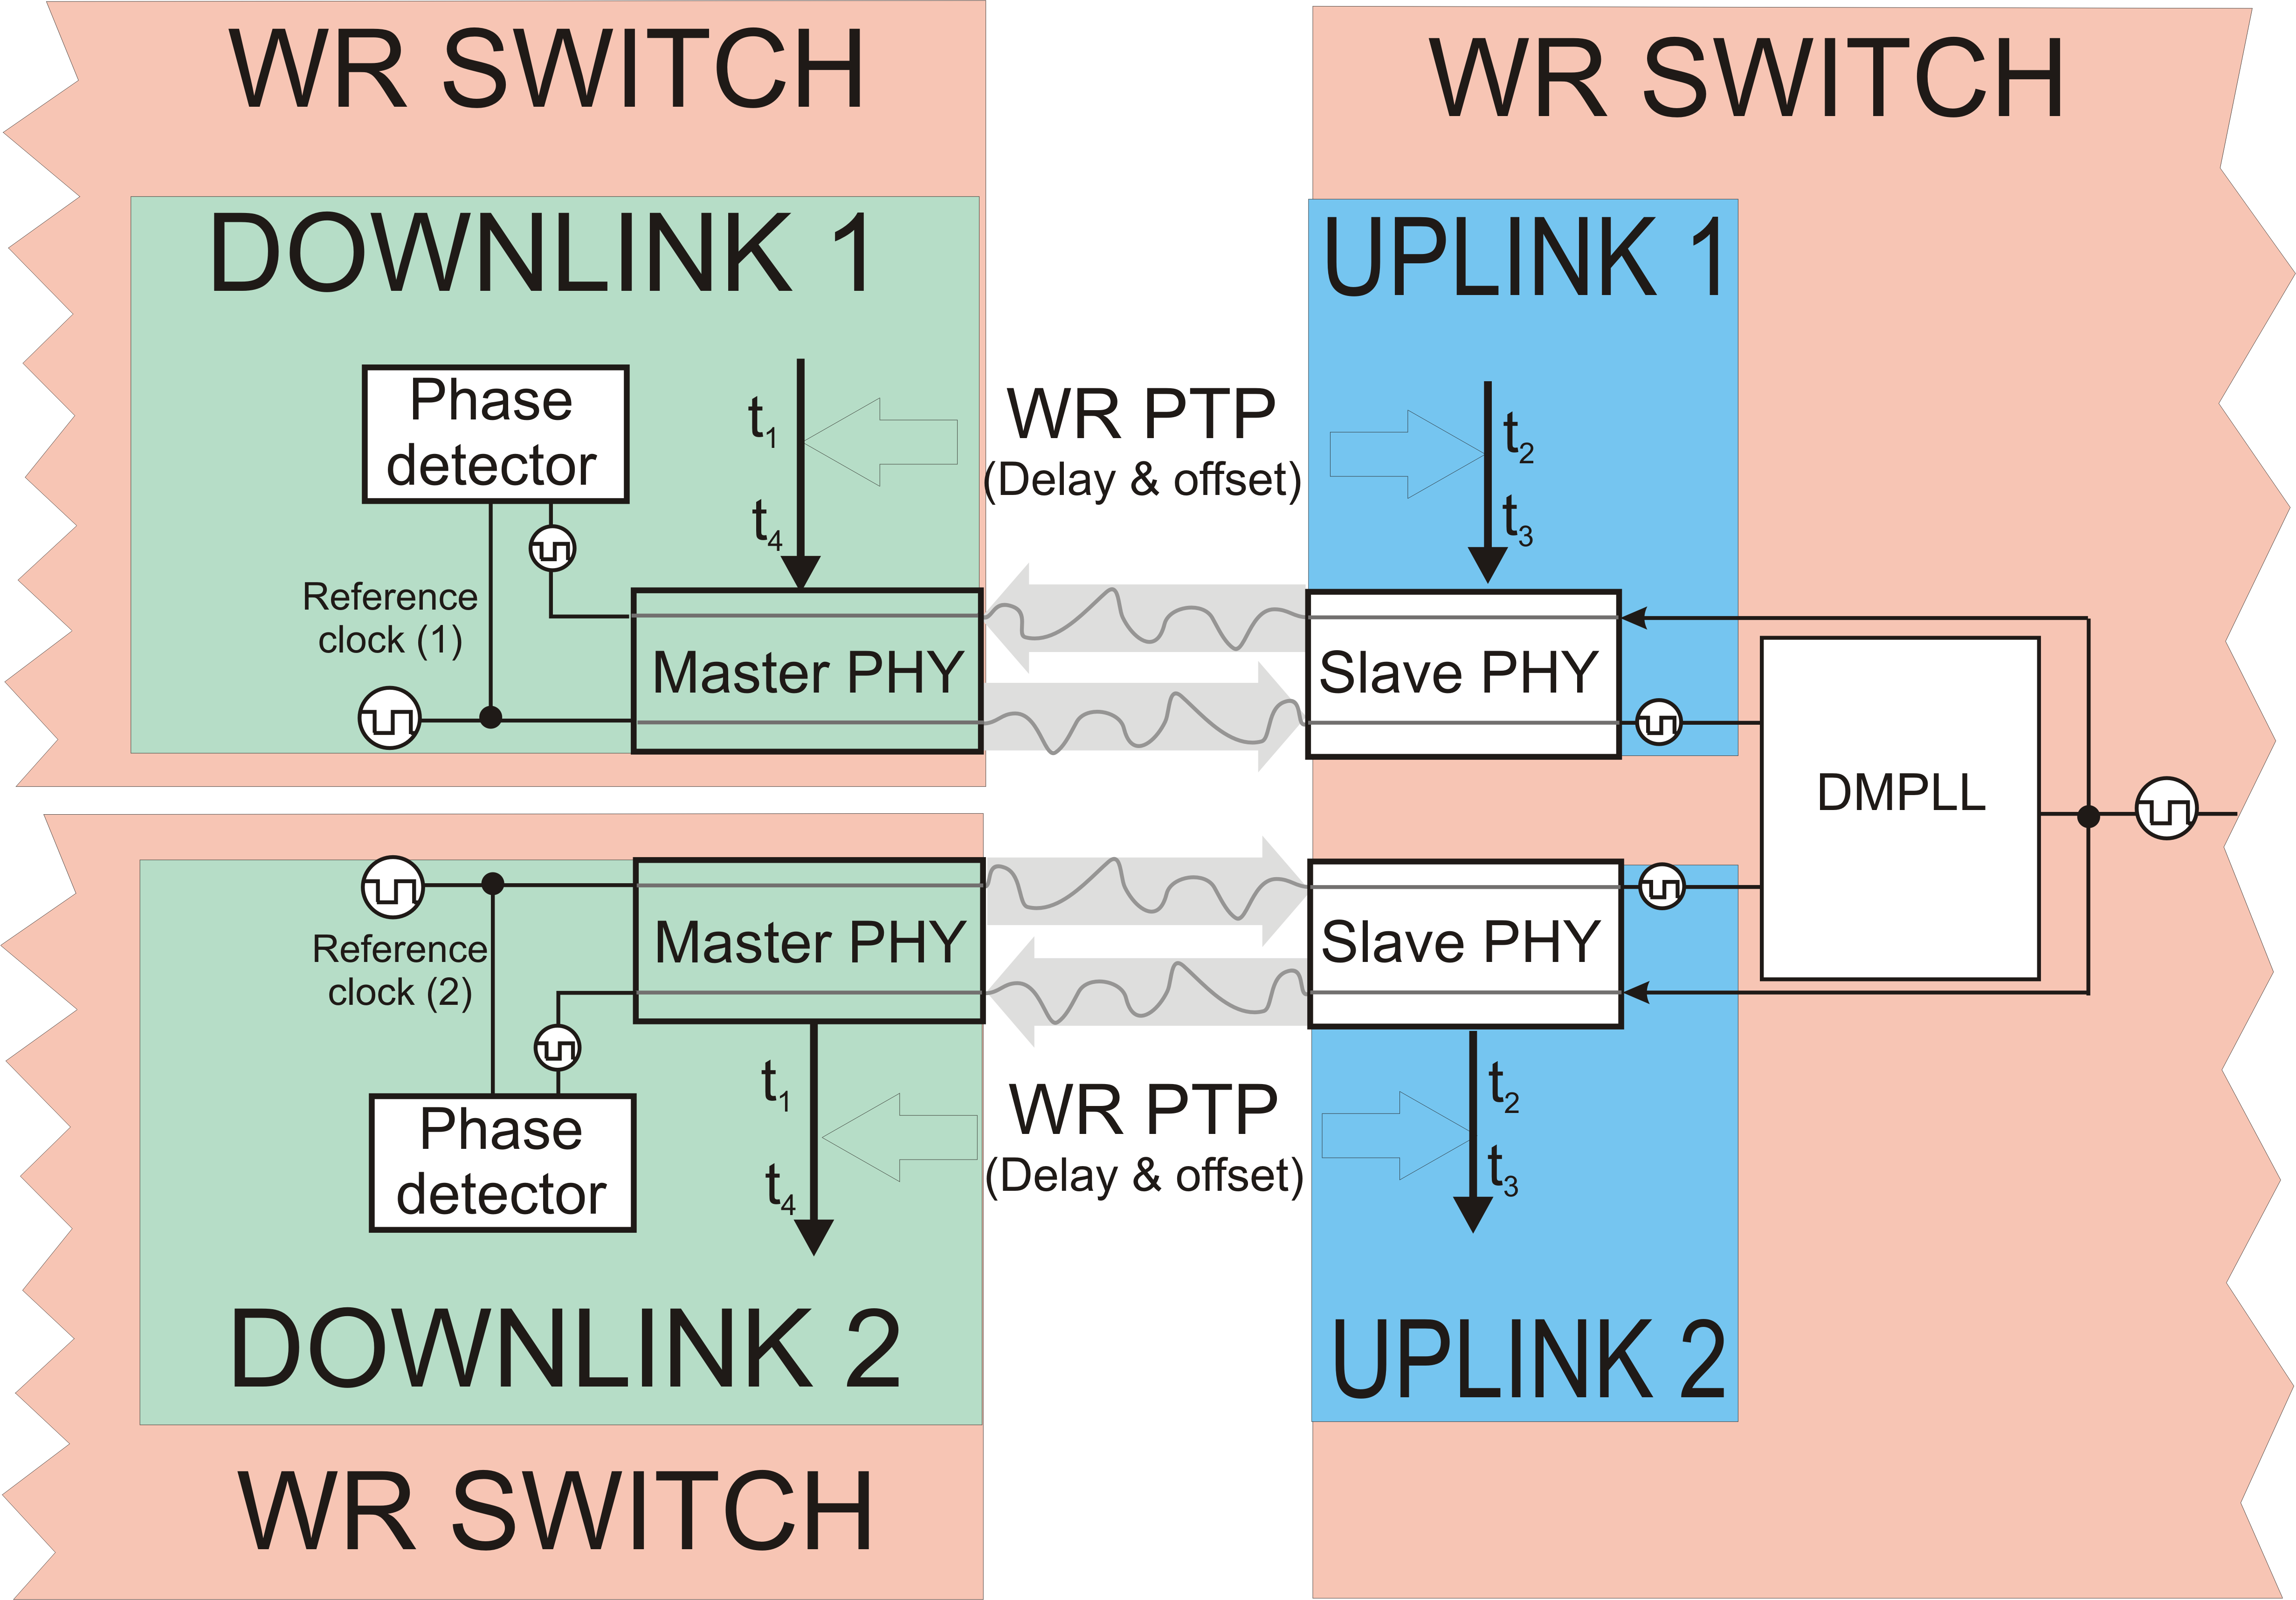
\includegraphics[height=6cm,keepaspectratio]{robustness/layer1redundancy2.png}

%  \includegraphics[height=6cm,keepaspectratio]{clockHoldover}


\end{figure}
\end{frame}
%\note[enumerate]       % Add notes to yourself that will be displayed when
%{                      % typeset with the notes or notesonly class options
%\item Note for Point 1   
%\item Note for Point 2   
%}


\subsection{Redundancy}

\begin{frame}
  \frametitle{Redundancy}
	\begin{itemize}
	\item MTBF = Mean Time Between Failures
	\item Probability of one particular unit of failing in a given day \footnote{Source: "Designing Large-Scale LANs"} :
	\begin{equation}
		P_= \frac{1 day}{2*MTBF}  
	\end{equation}
	
	\item Example MTBFs and probabilities of network units:
	  \begin{itemize}
	  \item Fiber connection: $MTBF=150 000h$; $p=0.0012\%$
	  \item Router : $MTBF=200 000h$; $p=0.0060\%$
	  \end{itemize}

	\end{itemize}
\end{frame}

\begin{frame}
  \frametitle{Redundancy in WR Network topology [1]}


\begin{figure}[tbp] % float placement: (h)ere, page (t)op, page (b)ottom, other (p)age
  \centering
  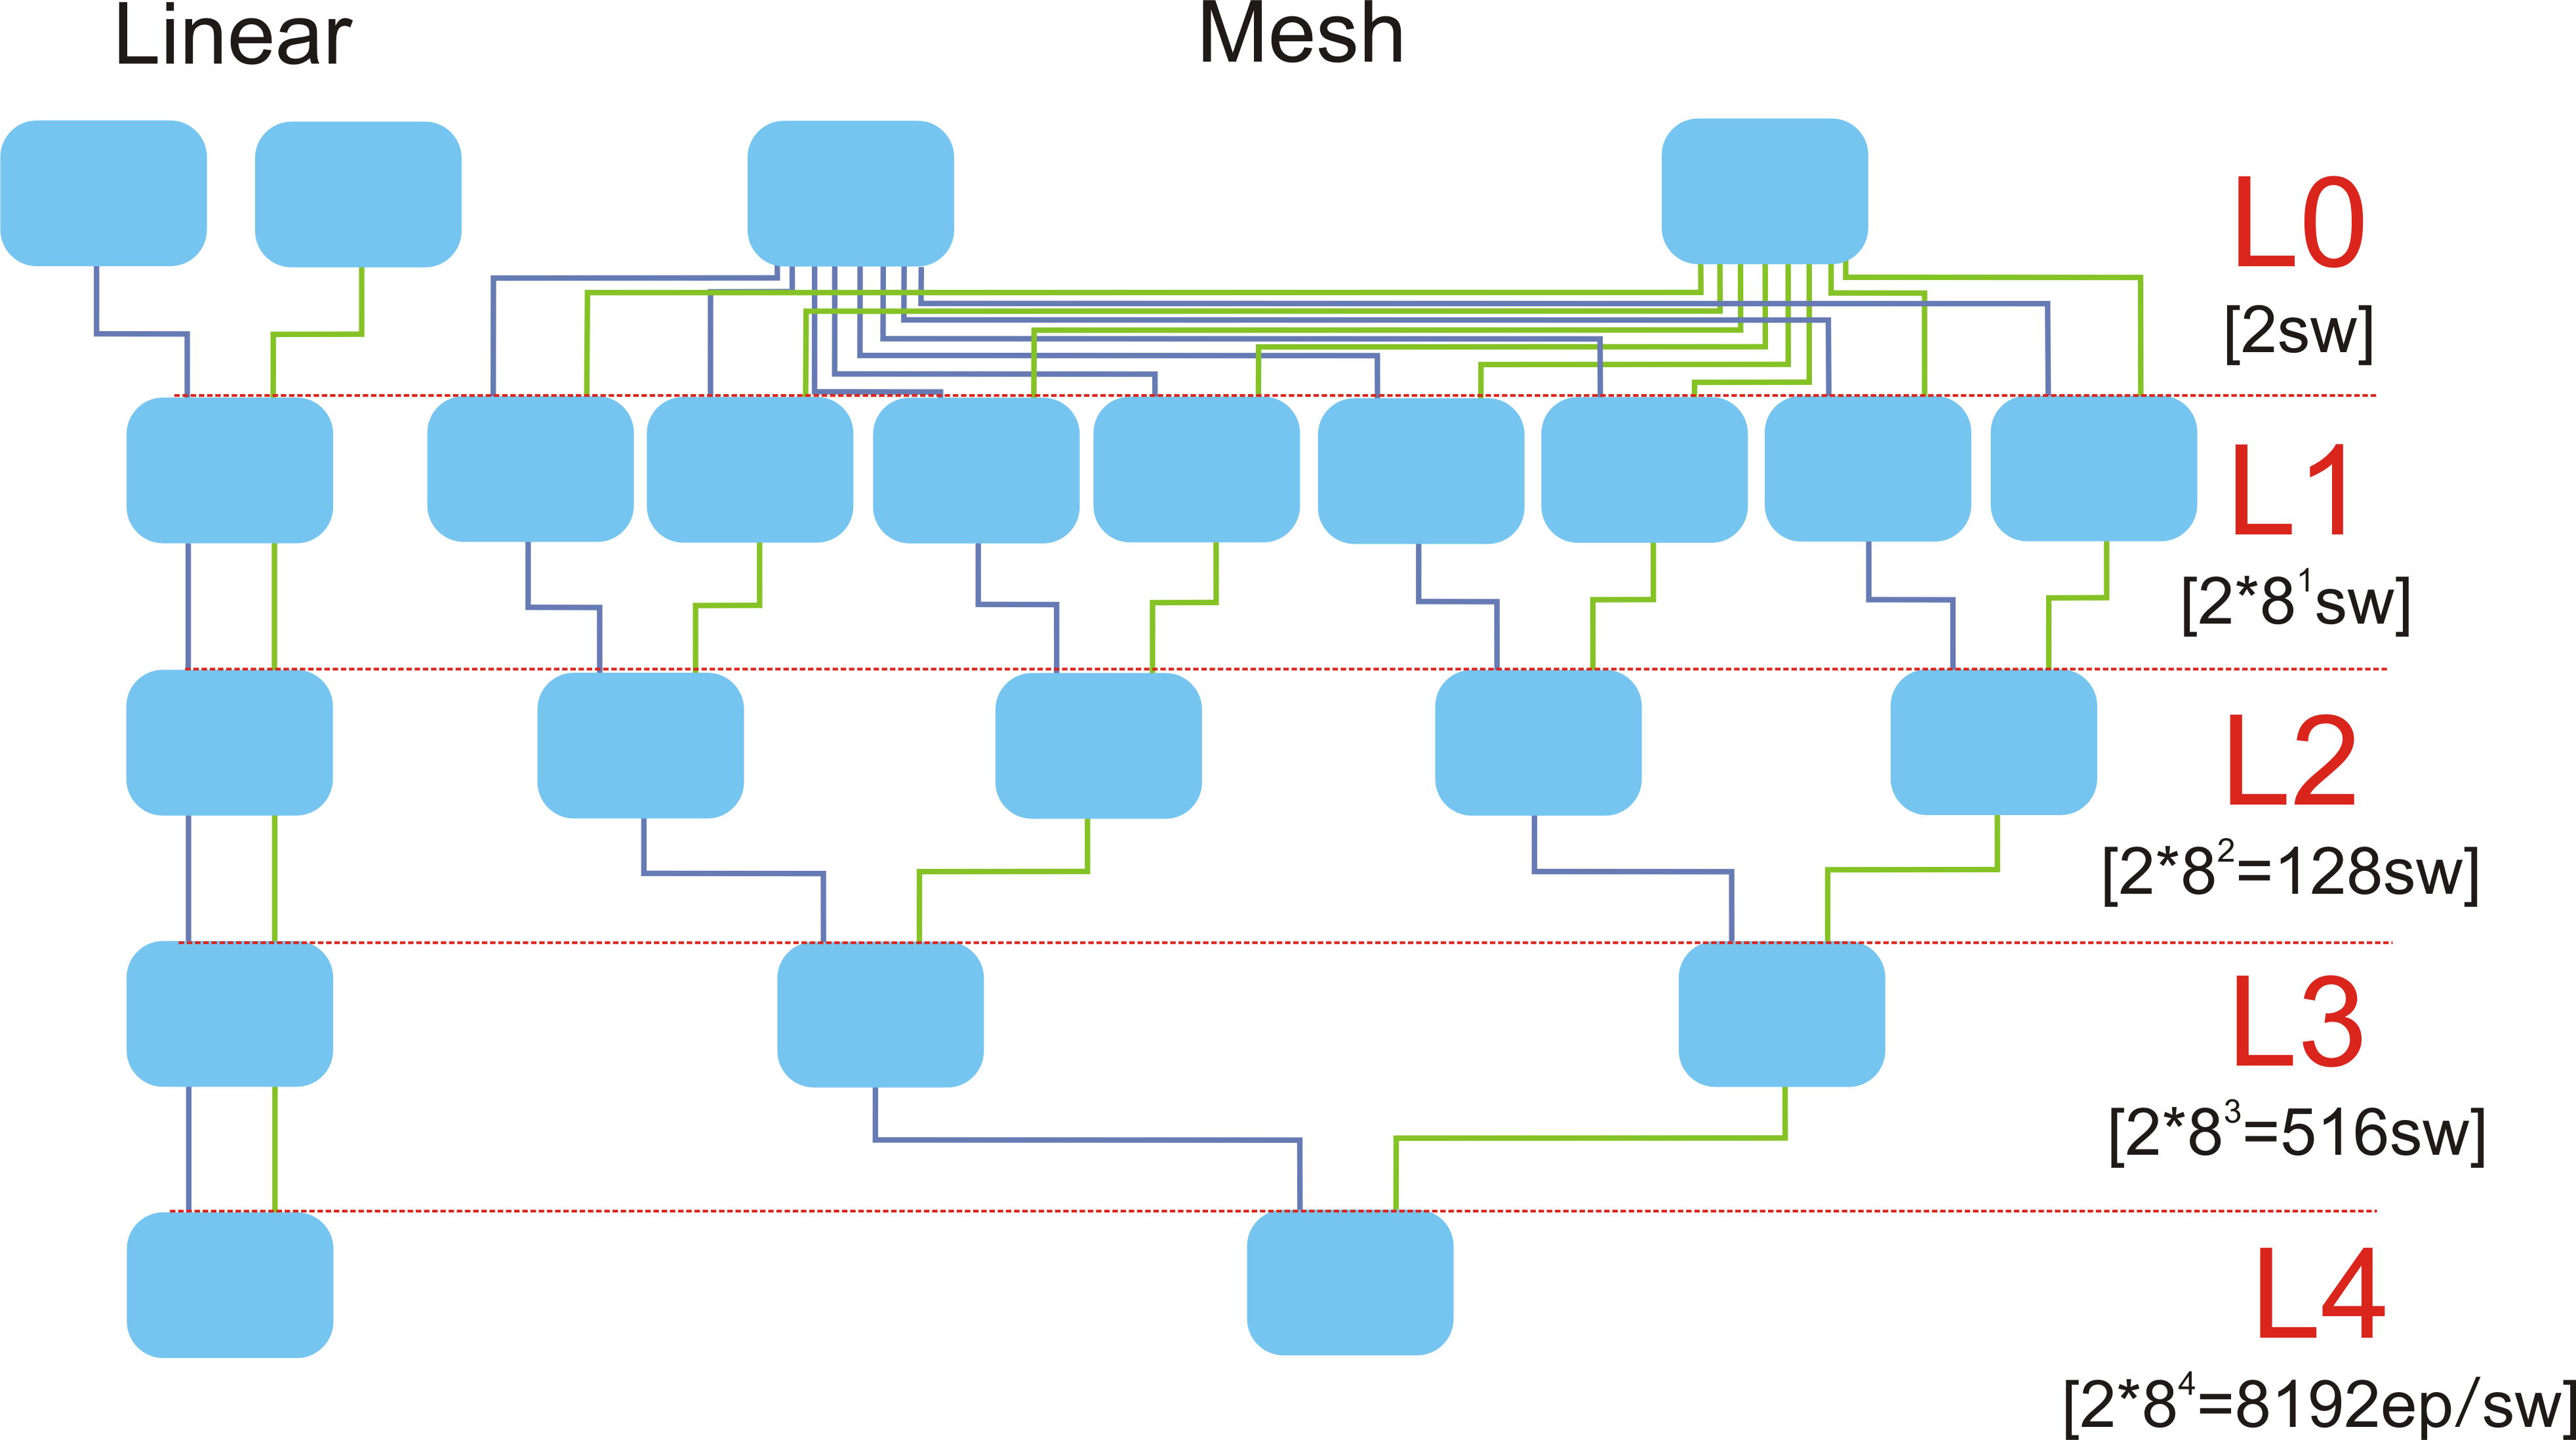
\includegraphics[width=9cm,keepaspectratio]{network/network_topology_0.png}

\end{figure}

$P=0.012\%$  \hspace{4cm}   $P=0.00000087\%$  \\   
$MTBF=16700[h]$ \hspace{2cm} $MTBF=1370000000[h]$ 

\end{frame}

\begin{frame}
  \frametitle{Redundancy in WR Network topology [2]}



\begin{figure}[tbp] % float placement: (h)ere, page (t)op, page (b)ottom, other (p)age
  \centering

  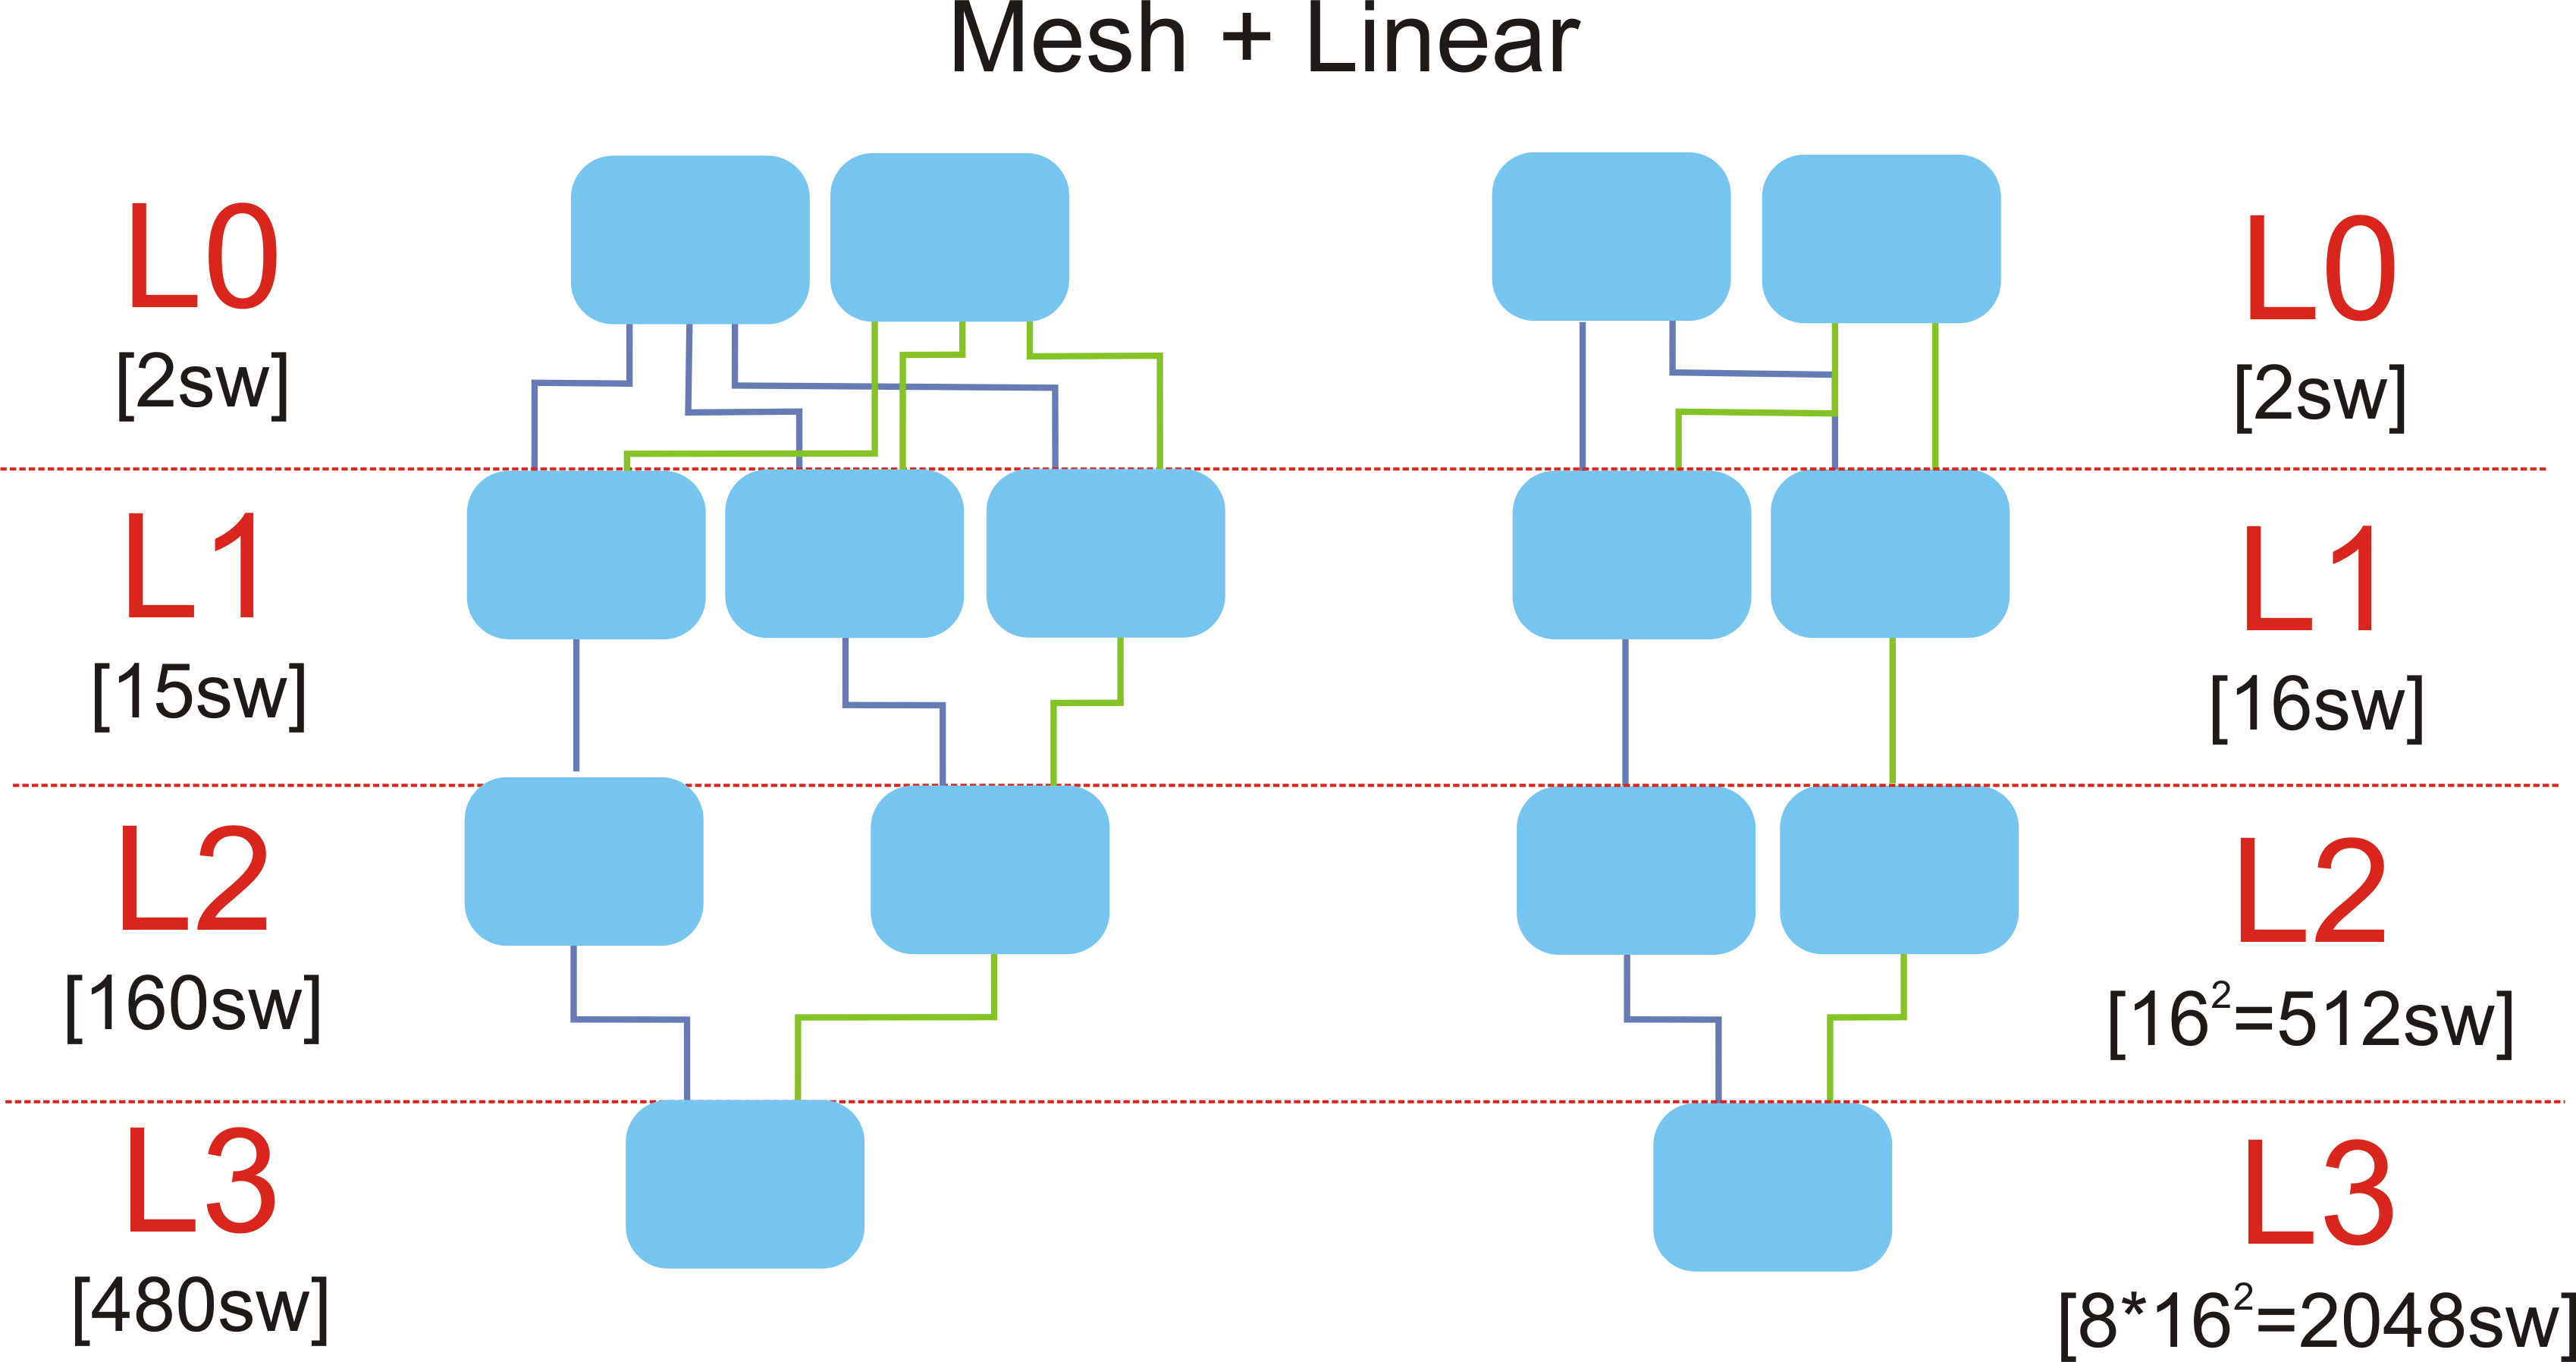
\includegraphics[width=9cm,keepaspectratio]{network/network_topology.png}

\end{figure}
\hspace{4cm}$P=0.00000154\%$    \\
\hspace{4cm}$MTBF=780000000[h]$ 

  \end{frame}




\section{Robustness Layer 2}

\subsection{Spanning Tree}
\begin{frame}
  \frametitle{Spanning Tree}   % Insert frame title between curly braces
  \begin{itemize}
	\item ST ensures a loop-free topology and broadcast radiation.
	\item WR Network needs ST to avoid loops created by the redundancy.
	\item Standard ST is slow, 1 min, Rapid Spanning Tree 6 seconds.
	\item Multiple (Rapid) Spanning Tree defines a SP for every defined VLAN
  \end{itemize}

Which Spanning Tree should I use? $\rightarrow$ It depends on the use case.

\end{frame}

\subsection{Jitter, Determinism and Network Dimension}

\begin{frame}
  \frametitle{Estimation of HP package transmision}   % Insert frame title between curly braces
  \begin{columns}[c]
  \column{3in}  % slides are 3in high by 5in wide
  \begin{itemize}
  \item Fiber link: measured 5$\mu$s/km
  \item Encoding/Decoding: estimated 120 cycles $\approx$ 2u$\mu$s per operation
  \item Sending: in worst case we need to finish sending current package, 1500 bytes $\approx$ 10$\mu$s
  \item Receiving: need to receive entire HP package, 500 bytes $\approx$ 4$\mu$s
  \item Routing = Sending + $\delta$ $\approx$ 11$\mu$s
  \end{itemize}

CERN: $\sim$40km; t$_{HP}$ $\approx$ 256$\mu$s [GW: 1000$\mu$s]
GSI : $\sim$4 km; t$_{HP}$ $\approx$  89$\mu$s [GW:  100$\mu$s]

  \column{3in}

  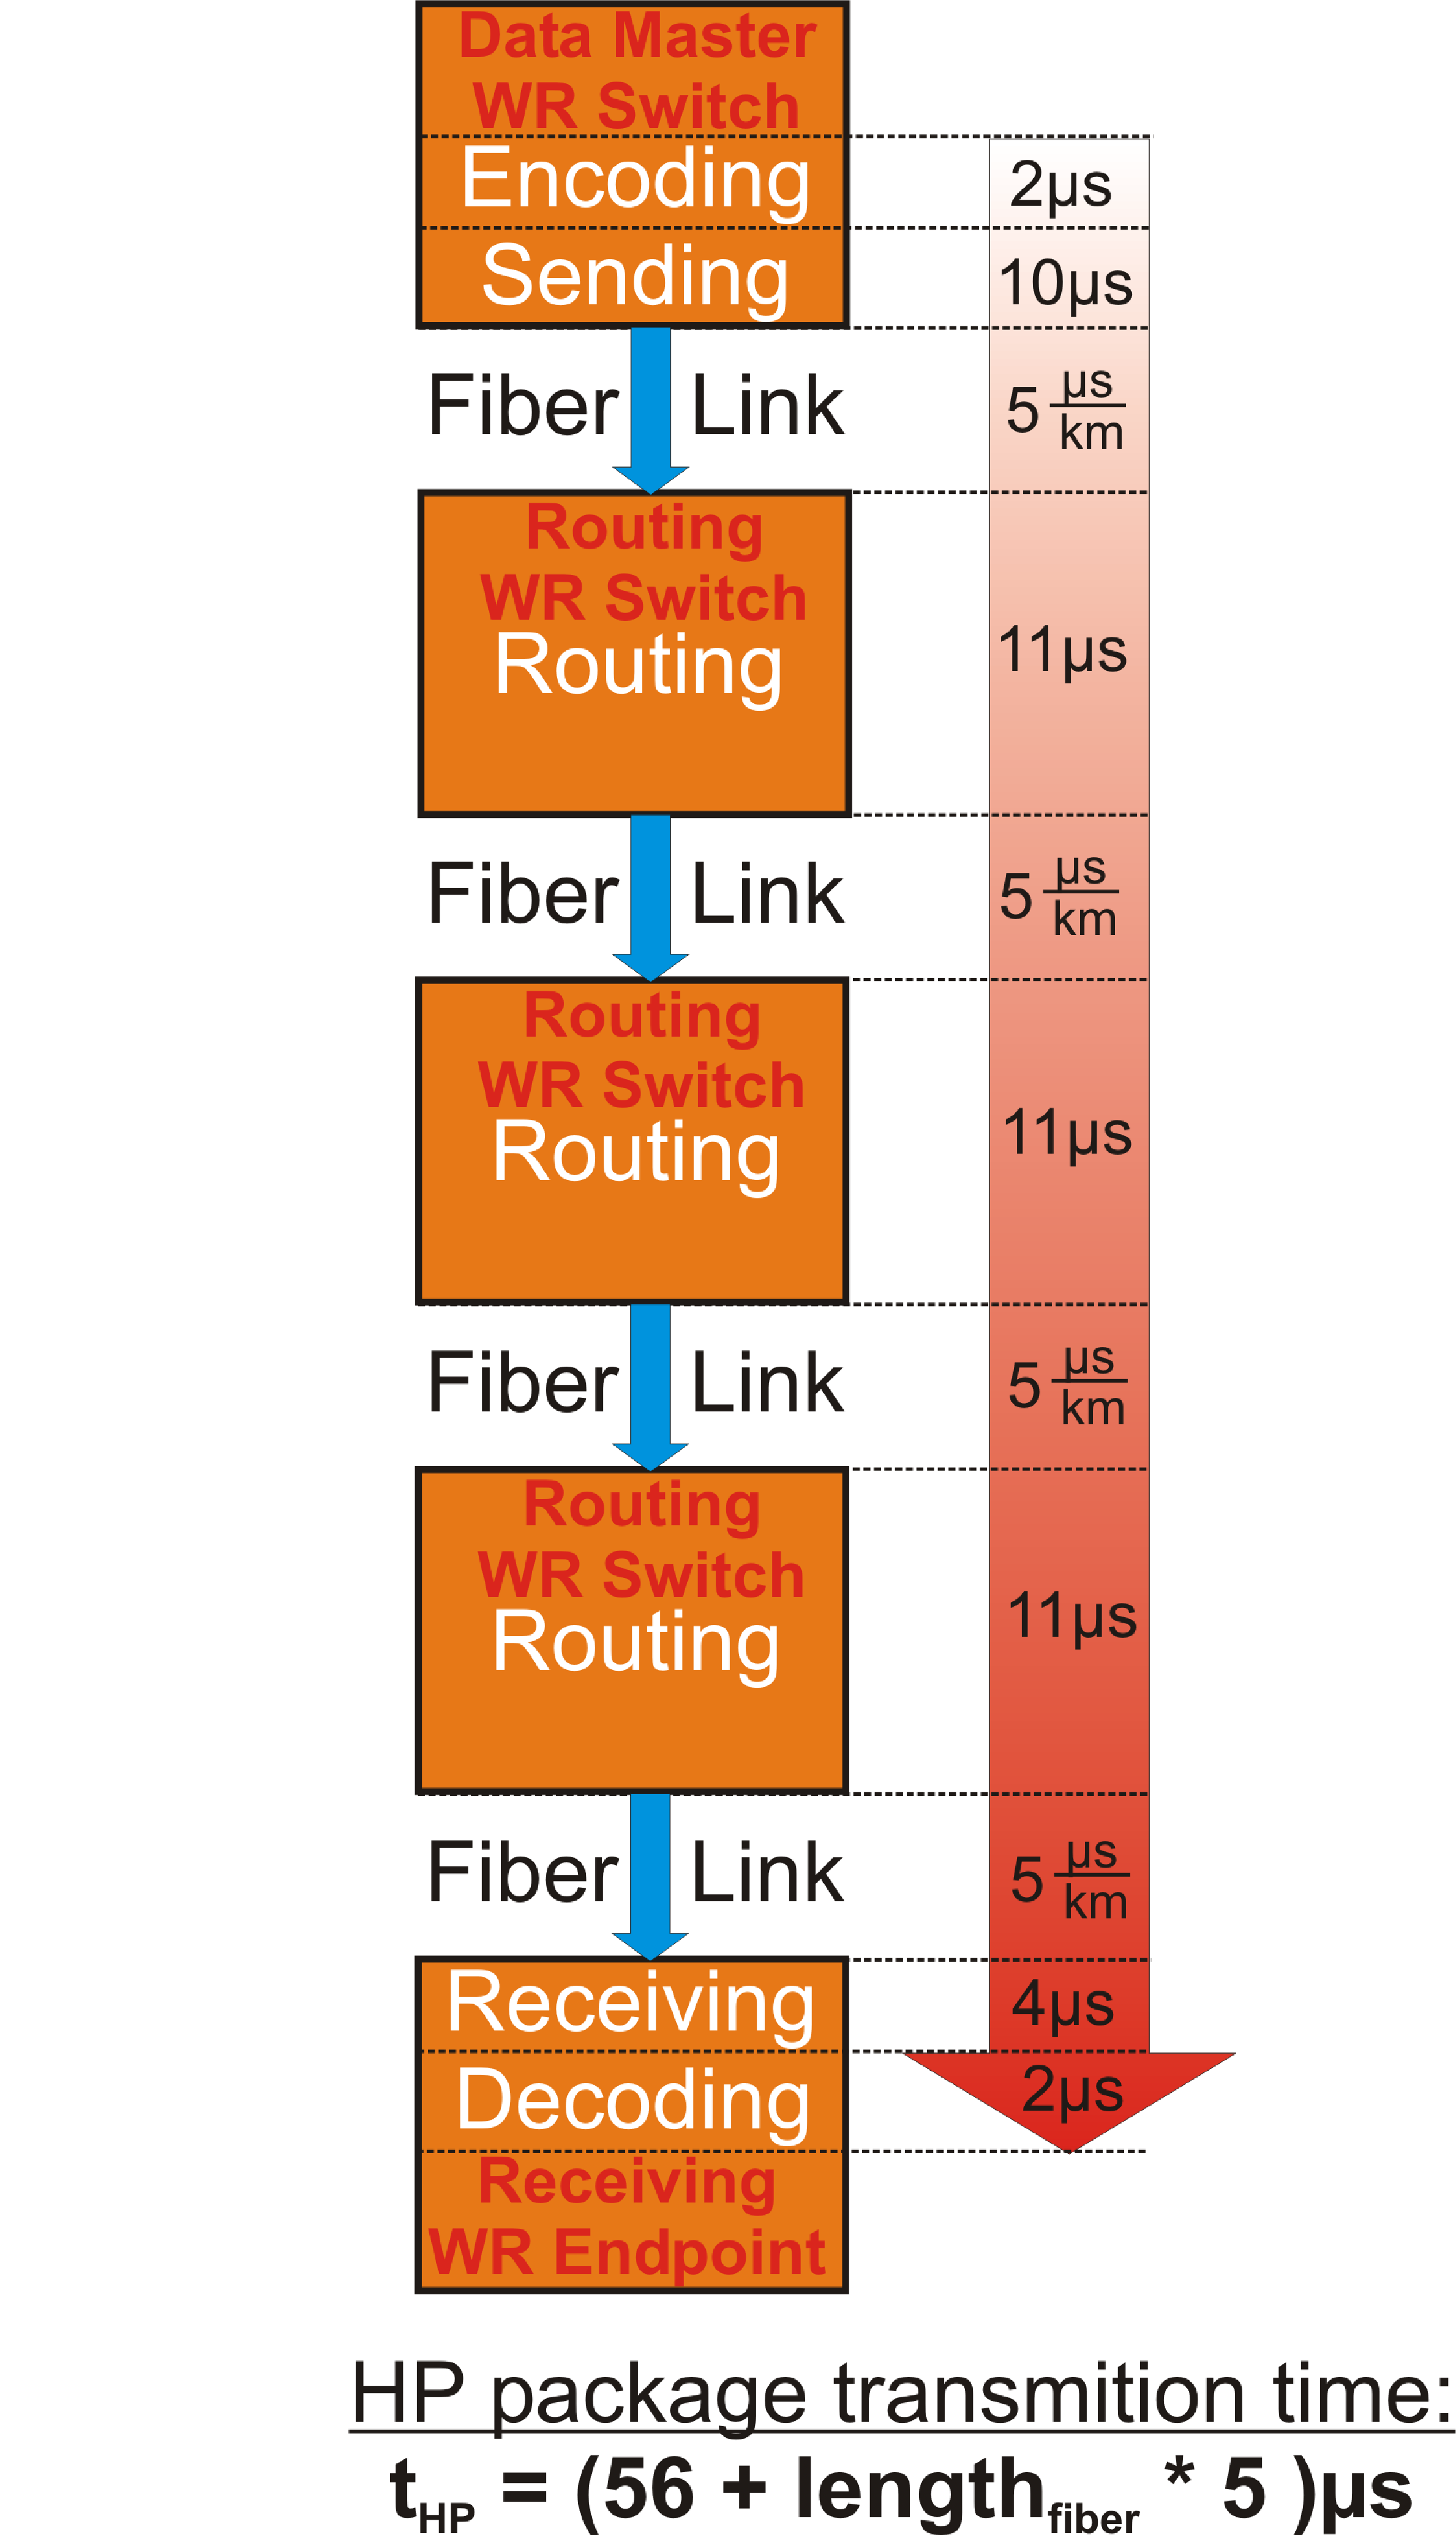
\includegraphics[height=6.2cm,keepaspectratio]{robustness/granuality_window}

  \end{columns}
\end{frame}

\section{Robustness Upper Layer}

\begin{frame}
  \frametitle{Robustness Upper Layer}   % Insert frame title between curly braces

  \begin{itemize}
  \item Congestion Control
  \item Forward Error Correction
  \end{itemize}
\end{frame}

\subsection{Congestion Control}

\begin{frame}
\frametitle{QoS, Flow Control and Congestion Control}

Quality of Service:
\begin{itemize}
\item WR Switches implements QoS in XX Class of Service, CS, (levels of priority) according to the IEEE 802.1 D/Q.
\item The highest priority, 7, is assigned to the Control Data Information.
\end{itemize}

Flow Control and Congestion Control
\begin{itemize}
\item WR needs a flow and congestion control scheme to keep the traffic below a level acceptable for the required performance.
\item The Management Master Nod, MMN, assigns to the node and each Class of Service, CS, a maximum throughput.
\item The WR Switch will supervise the traffic and inform to the MMN the correct throughput of the nodes.
\item If a node exceed the assigned throughput, the switch will drop the packets from the MAC address and CS of this node.
\end{itemize}
\end{frame}

\subsection{Forward Error Correction}
\begin{frame}
\frametitle{Broadcast and BER}
\begin{itemize}
\item Packets tagged with Priority 7 are broadcasted. 
\item The BER for Fiber Optic is $10^{-12}$ for Copper $10^{-9}$. 
\item By using broadcasting all the tree topology becomes, regarding the BER, a single cable...  
\end{itemize}

\begin{center}

\begin{columns}
  \begin{column}[c]{5cm}  % slides are 3in high by 5in wide
%	\includegraphics[height=6.2cm,keepaspectratio]{broadcast_ber.jpg}

	  % file name: E:/Moje Dokumenty/PW/doktorat/PhD_project/whireRabbit/repo/trunk/documentation/presentations/robustness/broadcast_ber.jpg
	  \includegraphics[width=6cm,keepaspectratio]{robustness/broadcast_ber.jpg}


  \end{column}

  \begin{column}[r]{5cm}  % slides are 3in high by 5in wide
Probability of Bit Error:
	\begin{equation}
		Pe_{system} = 1 - (1 - Pe)^{N{paths}} \nonumber 
	\end{equation}	    
	\begin{equation}
		Pe = BER \nonumber
	\end{equation}  
  \end{column}
 
\end{columns}

\end{center}

The BER for a 2000 nodes network and three layers of switches is:
\begin{itemize}
	\item Fiber Optic and Copper  Network, $2.10^{-7}$
	\item Fiber Optic Network,  $2.10^{-10}$
\end{itemize}
\end{frame}

\begin{frame}
\frametitle{Packet Erasure channel and Dropped Packets}

\begin{itemize}
	\item A Ethernet switching network, like WR, is a Packet Erasure Channel where the where packets are either received or lost.

\item According to IEEE 802.1 D, a packet will be always dropped by a \textbf{ switch} if it has a bit error, header or payload... 
\end{itemize}

Packet Error Rate throughout one year \footnote{Granularity Window $100\mu$}  $\approx$ $5.10^{-10}$

\end{frame}

\begin{frame}

\frametitle{Packet Erasure channel and Dropped Packets}

Always it is better a packet with an errors than no packet, isn't it?, Thus in WR network a packet will be dropped:

\begin{center}
	%\includegraphics[scale=0.30]{dropped_packet.jpg}
  \includegraphics[scale=0.30]{robustness/dropped_packet}


\end{center}
The WR Nodes will encode and decode the Control Information in to avoid loss of packets
\end{frame}

\begin{frame}
\frametitle{FEC Scheme}
The FEC overcomes two problems:
\begin{itemize}
	\item Loss of packets within the Switch-to-Switch paths, Erasure Codes.
	\item Errors in the packets, when they arrive to node. Linear Error-Correction Code.
\end{itemize}


Erasure Codes: 
\begin{itemize}
	\item Repetition code $\rightarrow$ Not enough!! 
	\item Reed Solomon 
	\item Low-Parity-Check-Code.
\end{itemize}
\end{frame}

\begin{frame}
\frametitle{FEC Scheme}
Linear Error-Correction Code:
\begin{itemize}
	\item Hamming Code
\end{itemize}

\vspace{0.5cm}
\begin{center}
WR FEC Scheme = Erasure Code + Hamming Code

Erasure Code  1/3 rate and 1 bit correction achieve $\approx 10^{-13}$   

\end{center}
\end{frame}




\begin{frame}
\frametitle{FEC Scheme}
Repetition Code Vs WR FEC Scheme
\begin{center}
%	\includegraphics[scale=0.35]{biterror.jpg}

  \includegraphics[scale=0.35]{robustness/biterror}



\end{center}
\end{frame}




\end{document}
